\chapter{Foot Placement Optimisation} \label{chap:optimisation}
The best possible anchor points for the supporting feet, given an initial point from the walking
gait state machine, must be found based on the heightmap. This is done by applying various
scores to the heightmap and selecting a point with the best score within an allowable
deviation from the initial point received from the gait state machine.

\section{Scoring} \label{sec:scores}
    The scores considered are the gradient and proximity scores. The gradient score aims to reject points with high gradients while the proximity score rejects points close
    to other parts of the terrain with steep inclines, i.e. to reject points inside holes or close to ledges.
    \subsection{Gradient Score}
        The gradient score is simply taken as the slope of the terrain at the current point. The aim of this score is to prevent the robot from slipping due to
        selecting anchor points with too steep of a gradient.
        
        As the heightmap slope is not defined by a known function, the gradient is calculated using the Sobel
        operator (\cite{sobel2014}), a combination of a central finite difference and a smoothing operator.
        
        \newpage
        \noindent
        Equation \ref{eq:sobelgx} and \ref{eq:sobelgy} describe the two separable x and y direction kernels, \(G_x\) and \(G_y\),
        of the Sobel operator. These kernels are a combination of central finite difference and smoothing operator, see Appendix \ref{app:sobel} 
        for a breakdown. Equation \ref{eq:sobelsg} combines \(G_x\) and \(G_y\) to produce the gradient score, \(S_g\). Note that these equations represent
        a single scalar result of the Sobel operator using the Frobenius inner product, \cite{horn2012matrix}. If evaluated over the whole heightmap this is equivalent
        to convolution.
        \begin{align}
            \begin{split} \label{eq:sobelgx}
                G_x(x,y) &= 
                        \sbox0{$
                        \begin{bmatrix}
                            +1 & 0 & -1\\
                            +2 & 0 & -2\\
                            +1 & 0 & -1
                        \end{bmatrix}
                        ,\boldsymbol{h}_{i,j}
                        $}
                        \mathopen{\resizebox{1.2\width}{1.1\ht0}{$\Bigg\langle$}}
                        \raisebox{0.08\ht0}{\usebox{0}}
                        \mathclose{\resizebox{1.2\width}{1.1\ht0}{$\Bigg\rangle$}}_{\mkern-10mu F}
            \end{split}\\[0.3cm]
            \begin{split} \label{eq:sobelgy}
                G_y(x,y) &= 
                        \sbox0{$
                        \begin{bmatrix}
                            +1 & +2 & +1\\
                            0 & 0 & 0\\
                            -1 & -2 & -1
                        \end{bmatrix}
                        ,\boldsymbol{h}_{i,j}
                        $}
                        \mathopen{\resizebox{1.2\width}{1.1\ht0}{$\Bigg\langle$}}
                        \raisebox{0.08\ht0}{\usebox{0}}
                        \mathclose{\resizebox{1.2\width}{1.1\ht0}{$\Bigg\rangle$}}_{\mkern-10mu F}
            \end{split}\\[0.3cm]
            S_g(x,y) &= C_g\sqrt{G_x(x,y)^2 + G_y(x,y)^2} \label{eq:sobelsg}
        \end{align}
        where,
        \[i = \big[\mkern-4.7mu\big[x-1,\mkern2mu x+1\big]\mkern-4.7mu\big]\]
        \[j = \big[\mkern-4.7mu\big[y-1,\mkern2mu y+1\big]\mkern-4.7mu\big]\]
        \noindent
        with \(C_g\) being the weighting constant associated with the gradient score, \(S_g\).
        
        \captionsetup[figure]{oneside,margin={0.9cm,0cm}}
        \begin{figure}[h]
            \centering
            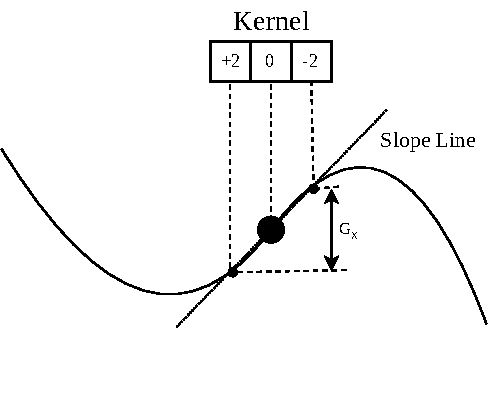
\includegraphics{slope_score.pdf}
            \caption{Slope Score}
            \label{fig:slope_score}
        \end{figure}

    \subsection{Terrain Proximity Score}
    The proximity score aims to bias the selected anchor point away from points near steep inclines in the terrain. This score is defined as the average of the height
    difference of the current point weighted by the gaussian kernel \(\boldsymbol{K}\), of size \(n\) by \(n\). The distance around inclines that is rejected depends on the the
    chosen size of the kernel \(\boldsymbol{K}\), the standard deviation of \(\boldsymbol{K}\) and the height differences. This score is described in Equation
    \ref{eq:terrain_prox}.

    \begin{equation} \label{eq:terrain_prox}
        S_p(x,y) = C_p\left|\frac{\sum\left\langle\boldsymbol{K},(\boldsymbol{h}_{i,j}-\boldsymbol{h}_{x,y})\right\rangle _{\mkern-3mu F}}{n^2}\right|
    \end{equation}

    \noindent
    where,
    \[i = \big[\mkern-4.7mu\big[x- \lfloor\tfrac{1}{2}n\rfloor,\mkern2mu x+\lfloor\tfrac{1}{2}n\rfloor\big]\mkern-4.7mu\big]\]
    \[j = \big[\mkern-4.7mu\big[y-\lfloor\tfrac{1}{2}n\rfloor,\mkern2mu y+ \lfloor\tfrac{1}{2}n\rfloor\big]\mkern-4.7mu\big]\]
    
    
    \noindent
    with \(x\) and \(y\) being the indices of the cell whose score is currently being evaluated, \(\boldsymbol{h}\) the
    heightmap and \(C_p\) the score's weighting constant.
    
    A diagrammatic, sliced, representation of the proximity score can be seen in Figure \ref{fig:prox_score_diagram}. The
    slice is taken along the x axis of the heightmap.

    \captionsetup[figure]{oneside,margin={0.9cm,0cm}}
    \begin{figure}[h]
        \centering
        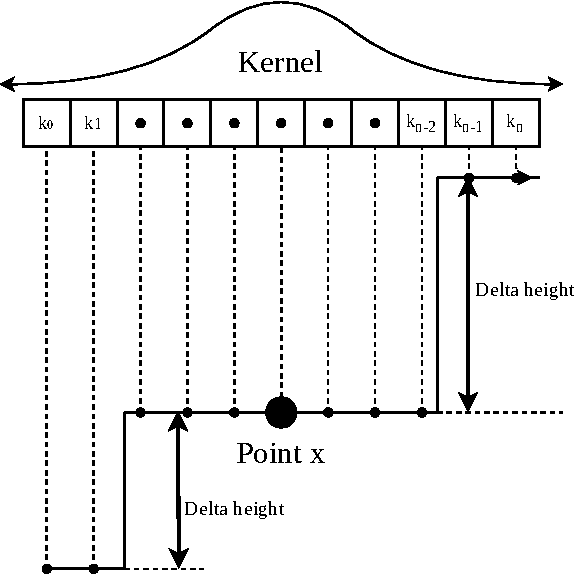
\includegraphics{prox_score.pdf}
        \caption{Proximity Score Diagrammatic Representation}
        \label{fig:prox_score_diagram}
    \end{figure}

    \subsection{Constraints}
    It is important to constrain the possible anchor points to confer to the stability triangle,
    meaning that the centre of mass of the robot must be inside the triangle formed by the three
    anchor points. Additionally, it is important that the points selected are not too far away,
    both in the horizontal and vertical direction for the robot to reach.


\section{Method of adjustment} \label{sec:radial_search}
    Once the heightmap has been processed into the score map, which is done by adding the
    slope score and terrain proximity score, the point with the best score must be found for every
    initial anchor point.
    The resolution of the heightmap is not very high and the adjusted anchor point is not
    allowed to deviate too far from the initial anchor point, additionally due to the parallel nature
    of the heightmap generation it is possible to score the entire heightmap with minimal cost.
    Thus, it was decided to not employ an optimisation algorithm, such as gradient decent or
    Bayesian, but rather to use a radial search algorithm. This algorithm progressively expands
    its searching radius over the square score grid until a valid score is found, at which point it
    terminates, thus ensuring that the closest valid point to the initial anchor point is selected.
    See Figure \ref{fig:score_search} for a diagram representing the search pattern for a 5 grid squares search area.
    Note that this search pattern will become inaccurate for large search areas, as the pattern steps
    in a square manner. This however is not much of a concern for smaller search areas.

    \captionsetup[figure]{oneside,margin={0cm,0cm}}
    \begin{figure}[h]
        \centering
        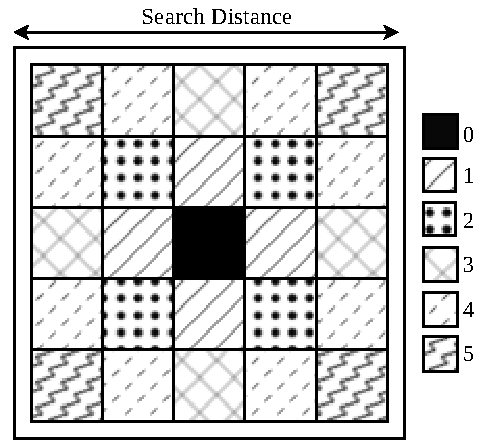
\includegraphics{search_diagram.pdf}
        \caption{Radial search, shown for a 5 cell search diameter.}
        \label{fig:radial_search}
    \end{figure}

    \section{Height Adjustment} \label{sec:height_adjust}
    After the horizontal position of the feet have been optimised, the height of the foot is simply set to the height of the
    terrain at the target horizontal coordinates. This ensures that the robots body remains level and at a constant global height.

    It is however important to adjust the reference floor height that the robot uses, if this is not done, then the robot will be
    incapable of surmounting terrain higher than its commanded standing height, as the robot will simply maintain said height and walk into the tall terrain.
    There are various methods to choosing a floor height, from using 
    a time of flight sensor underneath the robots main body to using height data from the heightmap.

    The method that was implemented in this paper uses the average of three highest target positions out of all the robots legs.
    This allows the robot to preemptively increase ore decrease its floor hight as it targets to step onto higher or lower terrain.

    \captionsetup[figure]{oneside,margin={0cm,0cm}}
    \begin{figure}[h]
        \centering
        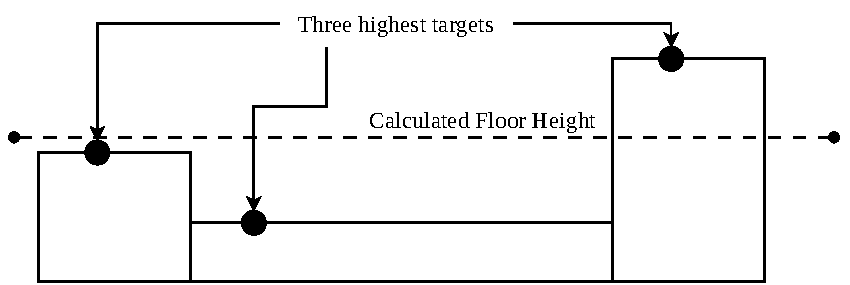
\includegraphics[width=\textwidth]{Diagrams-FloorHeight .drawio.pdf}
        \caption{Floor height diagram.}
        \label{fig:floor_height}
    \end{figure}

    While this method works well to preemptively adjust height and to optimise the body height against foot height, it does present one problem. If there is a tall piece of terrain in the path of the robots body
    without any feet positioned on it, then the robot will not adjust its body height to clear this piece of terrain. 
    Thus, the bounding box of the robots body, excluding the legs and feet, is checked against the heightmap
    and if anywhere in the bounding box is higher than the previously set floor height, the floor height is adjusted to this new value.